\documentclass[11pt]{article}

\usepackage[margin=1in]{geometry}
\usepackage{amsmath,amssymb}
\usepackage{booktabs}
\usepackage{graphicx}
\usepackage{tikz}
\usetikzlibrary{arrows.meta,positioning}

\title{thox-qk-rope: A Numerical Contract for Query-Key RMSNorm\\
and Rotary Embeddings in Local Decode}
\author{Craig Ross \and Tommy Xaypanya \\ THOX.ai LLC}
\date{4 November 2026}

\begin{document}
\maketitle

\begin{abstract}
THOX ships local language models whose attention blocks need two operators
that the published \texttt{thox-edge-ops} kernel does not implement:
per-head query-key RMSNorm, and NeoX rotary position embedding.
This note defines \texttt{thox-qk-rope}, a separate kernel with an
explicit numerical contract, a reference implementation, and a
kernel-builder source tree aimed at the Hugging Face kernel hub.
The contract follows the Qwen3 RMSNorm promotion rule and rotate-half
RoPE. The caller supplies the cosine and sine tables, so frequency
base, ABF, and YaRN stay outside the kernel and cannot drift from the
model fingerprint. The reference and a float32 C specification were
checked against an independent oracle. The CUDA and Torch bindings are
source only and have not been executed, so this note reports no device
speedup and no change to any published token rate. The kernel is a
companion to \texttt{thox-edge-ops}, not a replacement, and it does
not cover Gemma's unit-offset norm or interleaved rotary layouts.
\end{abstract}

\section{Introduction}

Local inference is the THOX default. A model that runs on a laptop, a
handset, or a small accelerator should not depend on a remote kernel
service to apply its attention arithmetic. The operators that sit on
that path are ordinary, and they are also where an eager implementation
spends launches: a norm, a rotation, a residual add, a gated
activation.

The public kernel \texttt{Thox-ai/thox-edge-ops} already targets the
residual RMSNorm and the SiLU-and-mul used by SwiGLU. Its card states
that Gemma's \((1 + w)\) normalization is out of scope, and it does not
list rotary embedding or query-key normalization. Two models on the
THOX Hugging Face organization make that gap concrete. The public card
for ThoxIOS-Edge-1.5B identifies the upstream architecture as
Qwen2.5-1.5B-Instruct, which uses rotary embeddings and does not use
query-key normalization. The public card for ThoxOpen-8B-Heretic
identifies the upstream architecture as Qwen3-8B. The Qwen3 technical
report, a vendor preprint, states that Qwen3 keeps the Qwen2.5 block
(grouped-query attention, SwiGLU, RoPE, pre-norm RMSNorm) and adds
QK-Norm while dropping the QKV bias~\cite{qwen3}.

This paper specifies the missing pair of operators and nothing else.
It does not claim a faster model, a qualified handset build, or a
change to either model card's measured token rate.

\section{Related work}

RMSNorm replaces the mean-subtraction of LayerNorm with the
root-mean-square of the activations and was introduced as a cheaper
normalization with comparable quality on the tasks in that
paper~\cite{rmsnorm}. Rotary position embedding encodes position as a
rotation so that the query-key inner product depends on relative
offset~\cite{rope}. Query-key normalization was introduced to stabilize
training of a 22-billion-parameter vision transformer; that work
normalized queries and keys, and the report's stability discussion is
about that training run rather than about an inference
kernel~\cite{vit22b}. Qwen3 cites that idea and implements the norm as
RMSNorm on the head dimension~\cite{qwen3}. We treat the Qwen3 report
as a vendor preprint. We do not treat its benchmark tables as THOX
results.

A public Hugging Face kernel, \texttt{sayakpaul/qk-norm-rope}, fuses an
RMSNorm taken across heads times head dimension with a split rotary
used by an audio-video diffusion transformer. The card reports a
\(5.75\times\) operator speedup against an eager sequence on an NVIDIA
GB10, and a small end-to-end change, for that diffusion workload. Those
figures are external, they describe a different reduction axis and a
different rotary layout, and they are not evidence about
\texttt{thox-qk-rope}.

Adjacent work on QK-normalized multi-head latent attention shows that a
dynamic per-token scale can be cached instead of a full key, and
reports a latency overhead under two percent on H800 in that paper's
own  runs~\cite{qkmla}. That design is about latent KV caches. We do
not implement it, and we do not adopt the overhead number.

\texttt{thox-edge-ops} version 1 is the THOX kernel this work sits
beside. Public metadata for the Metal build variant records kernel
commit \texttt{56b1c50} and kernel-builder commit \texttt{c212e38}.
The public card describes CUDA, Metal, and CPU backends and prints
operator timings. This paper does not re-measure those timings and does
not use them as a baseline for \texttt{thox-qk-rope}. A Hub filesystem
listing on 4 November 2026 returned one build directory,
\texttt{torch214-metal-aarch64-darwin}. We do not interpret that
listing as proof that other variants are absent from the kernel hub.

\section{Method}

\subsection{Where the kernel sits}

Figure~\ref{fig:place} shows one decoder block. \texttt{thox-edge-ops}
remains responsible for the pre-norm residual and for SwiGLU's
SiLU-and-mul. \texttt{thox-qk-rope} runs after the query and key
projections, on the head axis, and before attention. Value vectors are
not normalized and are not rotated.

\begin{figure}[t]
\centering
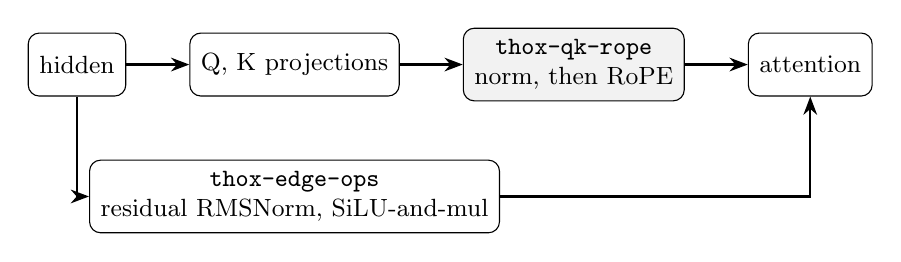
\begin{tikzpicture}[
  font=\small,
  box/.style={draw, rounded corners, align=center, inner sep=4pt, minimum height=8mm},
  arr/.style={-{Stealth}, thick}
]
\node[box] (h) {hidden};
\node[box, right=8mm of h] (proj) {Q, K projections};
\node[box, right=8mm of proj, fill=black!5] (op) {\texttt{thox-qk-rope}\\ norm, then RoPE};
\node[box, right=8mm of op] (attn) {attention};
\node[box, below=8mm of proj] (edge) {\texttt{thox-edge-ops}\\ residual RMSNorm, SiLU-and-mul};
\draw[arr] (h) -- (proj);
\draw[arr] (proj) -- (op);
\draw[arr] (op) -- (attn);
\draw[arr] (h.south) |- (edge.west);
\draw[arr] (edge.east) -| (attn.south);
\end{tikzpicture}
\caption{Placement. The new kernel does not replace \texttt{thox-edge-ops}. The value path skips both the norm and the rotation.}
\label{fig:place}
\end{figure}

\subsection{RMSNorm}

Let a row be \(x \in \mathbb{R}^{D}\) and the weight be \(w \in \mathbb{R}^{D}\). With \(\varepsilon \ge 0\),

\begin{equation}
\begin{aligned}
\bar{x}_i &= \mathrm{float32}(x_i), \\
s &= \Bigl(\frac{1}{D}\sum_{i=1}^{D} \bar{x}_i^{2} + \varepsilon\Bigr)^{-1/2}, \\
n_i &= \bar{x}_i \, s, \\
y &= w \odot \mathrm{cast}_{\mathrm{dtype}(x)}(n).
\end{aligned}
\end{equation}

The product uses the language's usual dtype promotion between \(w\) and the cast normalized row. This matches the Qwen3 module written as \texttt{weight * hidden.to(input\_dtype)}: a float32 weight and a float16 activation produce a float32 result; matched dtypes stay in that dtype. It is a different rule from a contract that casts after the weight multiply, or that casts before the multiply and then casts again. \texttt{thox-edge-ops} is a different operator and keeps its own rule. Golden files must not be shared between the two kernels.

The reduction is over the head dimension, not over all heads. That is the Qwen3 placement: the norm width is \texttt{head\_dim}~\cite{qwen3}.

\subsection{Rotary embedding}

The kernel implements NeoX rotate-half and no other layout. For an even rotary width \(R \le D\), split the prefix into halves \(a\) and \(b\) and let \(c, s\) be the caller-supplied tables, each of length \(R\):

\begin{equation}
\begin{aligned}
u &= a \odot c_{:R/2} - b \odot s_{:R/2}, \\
v &= b \odot c_{R/2:} + a \odot s_{R/2:}.
\end{aligned}
\end{equation}

The arithmetic is in float32. The stored dtype is the promotion of the activation dtype and the cosine dtype. Columns from \(R\) to \(D\) are copied. The kernel does not build frequencies. Base \(\theta\), ABF, YaRN, and the decision to duplicate each frequency into both halves belong to the caller. Qwen3's report states that the RoPE base was raised from \(10^{4}\) to \(10^{6}\) with ABF~\cite{qwen3}; a caller who wants that table constructs it before the launch.

If the activation is shaped \([B, S, H, D]\) and the table is shaped \([B, S, R]\), every head of a token shares the token's table. That is the layout of the Qwen3 projection after it is viewed onto the head dimension and before the transpose into attention. Applying the rotation on that view is the same map as applying it after the transpose, because the rotation does not mix heads or tokens.

\texttt{qk\_norm\_rope} applies Equation~(1), then Equation~(2). The reverse order is a different function and is not offered. Query and key weights are independent. Their head counts may differ. They share one cosine and sine table.

\subsection{What the source contains}

The repository holds:

\begin{itemize}
\item a NumPy reference that is the contract, including the float16 promotion cases;
\item \texttt{spec.c}, a float32 C implementation of the same index map, compiled and compared with the reference;
\item a Torch CPU binding and a CUDA binding over that float32 map, written for kernel-builder edition 6, not executed in this release;
\item a Metal shader fragment that is not listed in \texttt{build.toml} and is not a backend.
\end{itemize}

Native float16, bfloat16, and Metal stay out of the kernel card until a parity run exists. Interleaved GPT-J rotary is not implemented. Gemma's \((1+w)\) norm is not implemented.

The intended hub repository id is \texttt{Thox-ai/thox-qk-rope}, version 1. Until \texttt{kernel-builder upload} has been run on a locked toolchain, \texttt{get\_kernel} will not resolve that id. The source release and the binary release are different artifacts. Publishing source does not publish a binary.

\section{Evaluation protocol}

No THOX device measurement of this kernel exists. The protocol below is the gate for any later number. A number that skips a line is not a result of this kernel.

\begin{enumerate}
\item Device, GPU or CPU identifier, driver, PyTorch build, and the kernel-builder lock.
\item Operator parity against the NumPy reference on float32 for head dimensions 64 and 128; rotary width equal to the head dimension; rotary width 64 with a copied tail; batch and sequence greater than one; sequence length 1; distinct query and key head counts.
\item Maximum absolute error, not a single averaged tolerance.
\item If a timing is reported: warmup, number of iterations, the eager program it is compared with, whether the cosine table is included, and the median. A kernel-only ratio is not a tokens-per-second claim.
\item An end-to-end claim additionally names the model revision, the quant, the runtime, the context, and cold versus warm. The 35.67 tokens per second figure on the ThoxIOS-Edge-1.5B card is a measurement of that packaged configuration on a 4-vCPU host, dated 31 October 2026. It is not a measurement of \texttt{thox-qk-rope}.
\end{enumerate}

\section{Security and deployment}

The kernel takes activations and a position table. It does not deserialize pickled tensors, open a socket, or read a credential. The Python reference is local NumPy. A hub binary, once it exists, should be consumed through the kernel lockfile and an offline download, the same pattern \texttt{thox-edge-ops} documents, so a machine that is not allowed to fetch code at inference time does not fetch code at inference time.

RoPE tables are not a cache key. Anyone who later stores a KV cache must still bind that cache to the principal and to the exact model fingerprint: weights, quant, tokenizer, RoPE parameters, layout, and engine. This kernel does not store a cache and does not relax that rule. A norm of queries and keys is not semantic memory.

\section{Limitations}

The CUDA and Torch CPU sources are unread by a compiler in this release. A transcription error against \texttt{spec.c} would not have been caught. Float32 is the only native dtype. Metal is a note. There is no backward pass. There is no claim about Jetson sm\_87 until the builder's capability list is shown to include it; the build file does not pin a capability list, so the builder default is what a future binary will contain.

Partial rotary copies the tail after the norm. Models that rotate before they normalize, or that normalize only the rotary slice, are outside the contract.

\section{Conclusion}

\texttt{thox-qk-rope} is the attention-preparation companion to \texttt{thox-edge-ops}. The contract is Qwen3's RMSNorm promotion followed by caller-supplied NeoX RoPE, checked for the reference and for a float32 C specification. The hub binary is a later, gated build. No speedup is claimed.

\section*{Reproducibility}

The source tree contains \texttt{tests/test\_reference.py} and \texttt{tests/test\_spec.py}. From the repository root, \texttt{python3 -m unittest tests.test\_reference tests.test\_spec -v} runs the oracle checks and compiles \texttt{spec.c} with the host C compiler. No network, GPU, or package install is required beyond NumPy and a C11 compiler. \texttt{example.py} prints shapes only.

\section*{Generative AI assistance}

Drafting assistance was provided by Grok, a generative model operated by xAI. The human authors are responsible for the claims, the citations, and the decision to publish. The model is not an author.

\begin{thebibliography}{9}

\bibitem{rmsnorm}
B.~Zhang and R.~Sennrich.
Root mean square layer normalization.
\textit{arXiv}:1910.07467, 2019.

\bibitem{rope}
J.~Su, Y.~Lu, S.~Pan, A.~Murtadha, B.~Wen, and Y.~Liu.
RoFormer: Enhanced transformer with rotary position embedding.
\textit{arXiv}:2104.09864, 2021.
Also \textit{Neurocomputing}, vol.~568, 127063, 2024.

\bibitem{vit22b}
M.~Dehghani \emph{et al.}
Scaling vision transformers to 22 billion parameters.
\textit{arXiv}:2302.05442, 2023.
Proceedings of ICML, PMLR 202, 2023.

\bibitem{qwen3}
Qwen Team.
Qwen3 technical report.
\textit{arXiv}:2505.09388, 2025.
Vendor preprint.

\bibitem{qkmla}
Y.~Han, Y.~Zhao, J.~Zhou, L.~Li, and R.~Sun.
QK-normed MLA: QK normalization without full key caching.
\textit{arXiv}:2606.16310, 2026.
Preprint. Figures in that paper are not THOX results.

\end{thebibliography}

\end{document}
